\documentclass[12pt, letterpaper]{article}
\usepackage[utf8]{inputenc}
\usepackage{amssymb}
\usepackage{amsmath}
\usepackage{graphicx}
\usepackage{float}
\usepackage{indentfirst}
\usepackage[ruled,vlined]{algorithm2e}
\SetKwComment{Comment}{$\triangleright$\ }{}

\title{Algoritmo de Recocido Simulado para el problema del Agente Viajero}
\author{Juan C. Castrejón}
\date{Mayo 2019}

\begin{document}

\maketitle
\newcommand{\R}{\mathbb{R}}
\renewcommand{\abstractname}{Resumen}
\renewcommand{\algorithmcfname}{Procedimiento}
\renewcommand{\refname}{Referencias}
\renewcommand{\figurename}{Figura}

\begin{abstract}
En la mayoría de los problemas de optimización, encontrar \textit{la mejor solución} o \textit{solución óptima}, usualmente es una tarea no trivial. Cuando se está tratando con problemas de este tipo, se puede recurrir a técnicas llamadas heurísticas, las cuales en muchas ocasiones están inspiradas por fenómenos que ocurren en la naturaleza.
\par
En este documento se aplica el algoritmo de recocido simulado, un algoritmo de busqueda metaheurística para encontrar de manera efectiva soluciones aproximadas a la óptima, en el problema del agente viajero.
\par
Se proporcionan resultados comparativos de la ejecuión con diferentes parámetros.
\end{abstract}


\section{Introducción al problema}

Dado un conjunto de ciudades y la distancia entre cada par de ciudades, el problema del agente viajero, consiste en buscar la ruta más corta que visita cada ciudad exactamente una vez y regresa al punto de partida. Este es un problema clasificado como NP-duro (no se conoce una solución en tiempo polinomial). A partir de este momento se referirá al problema como TSP (Traveling Salesman Problem) por sus siglas en inglés. Se verifica la solución trivial en el procedimiento \ref{proc:1}.

\LinesNumbered
\begin{algorithm}[H]
Sea $\{1, 2, 3, ..., n\}$ el conjunto de ciudades.\\
Considerar la ciudad 1 como punto de partida.\\
Generar todas las $(n - 1)!$ permutaciones de ciudades.\\
Calcular la distancia de cada permutación y mantener la de menor costo.\\
Regresar la permutación de menor distancia.\\
\caption{Solución trivial de TSP}
\label{proc:1}
\end{algorithm}
\LinesNotNumbered
\bigskip

La complejidad de esta aproximación está dada por $O(n!)$ (el factorial del número de ciudades), lo que la vuelve impráctica incluso para conjuntos con sólo 20 ciudades.
\par
La necesidad de encontrar una solución rápidamente a problemas donde los métodos conocidos son muy lentos, como TSP, es lo que nos lleva al estudio de las \textit{heurísticas}.

\section{Heurísticas y Metaheurísticas}

Las heurísticas son un método de solución de problemas, que usa técnicas que han sido adaptadas al problema para obtener ventaja de la información disponible, con el fin de producir soluciones \textit{suficientemente buenas}, no necesariamente óptimas, de forma \textit{rápida}. Una heurística a menudo involucra elementos aleatorios, por lo que no puede probarse que es capaz de encontrar todas las soluciones a un problema.
\par
Una metaheurística es una técnica independiente del problema que se basa en explorar más profundamente el espacio de soluciones y con suerte obtener una \textit{mejor solución} (que en ocasiones coincide con la óptima).
\par
Un ejemplo de una heurística para TSP, es el uso del algoritmo glotón (\textit{greedy} en inglés), el cual encuentra una \textit{buena}, pero no óptima, solución en un tiempo razonablemente corto. La heurística se basa en elegir en cada paso la ciudad más cercana, independientemente de si esta desición afecta buenas elecciones en pasos posteriores.
\par
El algoritmo de \textit{recocido simulado} es una metaheurística cuyo objetivo es encontrar, mediante búsqueda \textit{inteligente}, una buena aproximación al valor óptimo de una función en un espacio muy grande; en el caso de TSP, encontrar una ruta cuya distancia es cercana a la óptima. El funcionamiento y la efectividad de este algoritmo será estudiado en las siguientes secciones.

\section{Función de costo}

Requerimos un mecanismo para verificar que una solución es mejor que otra. A este mecanismo se le conoce como función de costo, la cual relaciona una solución actual del problema con un número real, esto permite la comparación de soluciones. Sea $s=\{c_1,...,c_n\}$ una solución a un problema de TSP con $n$ ciudades. La función de costo $f$ de $s$ se define como:

\begin{equation}
f(s)=\sum_{i=2}^{n}w(c_{i-1}, c_i)    
\end{equation}

donde $w$ es la función que calcula la distancia entre dos ciudades. Por lo que la función de costo es simplemente, la suma de las distancias entre las ciudades de $s$.
\par
Sea $S$ el conjunto de posibles soluciones para una instancia de TSP. Sean $s_1, s_2 \in S$, decimos que $s_1$ es mejor que $s_2$ si $f(s_1) < f(s_2)$. La función de costo puede ser normalizada para facilitar identificar soluciones factibles; el hecho de que una solución pueda ser no factible, es discutido en la sección \ref{sec:1} (Gráfica completa).

\section{Recocido Simulado}

La inspiración y nombre para este algoritmo proviene del procedimiento de recocido en metalurgia. Esta técnica se basa en calentar y enfriar controladamente un material, para aumentar su ductilidad y que sea más fácil de trabajar. De manera similar el algoritmo permite el enfriamiento lento y controlado de la temperatura del sistema, donde la el decremento lento de la temperatura es interpretado como la probabilidad de aceptar peores soluciones comparadas con una mejor solución global conocida. Aceptar peores soluciones es una propiedad fundamental de las metaheurísticas porque permite una exploración más extensiva en la búsqueda de la solución óptima.
\par
La idea general del algoritmo es comenzar con una temperatura inicial $T_0$ y una solución inicial $s_0$, obtenidos de \textit{alguna forma} (ver subsección \ref{sub:2}).
\par
Se establece un número $L$ que será el tamaño de los lotes que se deberán completar \textit{aceptando} soluciones vecinas a partir de la solución $s_0$.
\par
En cada paso, la mejor solución encontrada por la función $vecino()$ (descrita en la subsección \ref{sub:1}) es guardada globalmente con el fin de mantener la mejor solución encontrada; y cualquier solución $s'$ \textit{aceptada} en un lote, es guardada para generar las siguientes soluciones vecinas ($vecino(s')$).
\par
Al completar un lote y cumplir otras condiciones, la temperatura $T$ del sistema disminuye lentamente, hasta cumplir la condición de terminación descrita en la siguiente subsección.
\par
El algoritmo realiza la búsqueda permitiendo que una solución \textit{peor} a la actual sea \textit{aceptada} y usada para crear nuevas soluciones a partir de ésta; donde cada vez que la temperatura $T$ disminuye, la aceptación de soluciones será cada vez más estricta, lo que ocasiona que el espacio de busqueda se reduzca poco a poco, pero también permite escapar de alguna búsqueda en la que tal vez ya no se puede mejorar la solución, usando los vecinos actuales.

\subsection{Aceptación por umbrales}

Dadas una temperatura $T \in R^+$, una solución $s \in S$ y $s'$, una solución vecina de $s$ obtenida de forma aleatoria, decimos que $s'$ es aceptada si $f(s') < f(s) + T$. En caso de ser aceptada, actualizamos $s$ para que sea $s'$ y continuamos mientras la temperatura $T$ es disminuida lentamente. El proceso termina cuando $T < \epsilon$ (para $\epsilon > 0$ muy pequeña).

\subsection{Vecino}
\label{sub:1}

Dada una solución $s \in S$, decimos que $s'$ es vecino de $s$ si a partir de s, se generó de manera aleatoria con distribución uniforme, una permutación $s'$ donde se intercambiaron dos ciudades de $s$. Basado en lo anterior, $vecino(s)$ es la función que regresa un vecino de $s$.

\subsection{Lotes}

Un lote será un número determinado de soluciones aceptadas. Los lotes servirán para establecer las condiciones que decrementarán la temperatura $T$. Los procedimientos \ref{proc:2} y \ref{proc:3} muestran la forma en la que las soluciones son aceptadas en lotes y la temperatura decrementa conforme se completan los lotes.
\par
Nótese que $CalculaLote(T,s)$ puede nunca terminar, debido a que se requiere un número $L$ de soluciones aceptadas para completar el lote, y éstas pueden no existir o jamás ser encontradas, por lo que se requiere una medida de escapar del \textbf{while}. En este caso se usará un número $M$ que indica el número máximo de intentos para completar el lote.

\begin{algorithm}[H]
\SetKwProg{Fn}{procedure}{}{}
\Fn(\Comment*[f]{Temperatura $T$, solución $s$}){CalculaLote(T, s)}{
    $c \gets 0$\\
    $r \gets 0.0$\\
    $i \gets 0$\\
    \While{$c < L$} {
        $s' \gets vecino(s)$\Comment*[f]{Función que obtiene un vecino de $s$}\\
        $i \gets i+1$\\
        \If(\Comment*[f]{Aceptamos la solución vecina}){$f(s') \leq f(s) + T$}{
            $s \gets s'$\\
            $c \gets c+1$\\
            $r \gets r+f(s')$\\
        }
        \If(\Comment*[f]{Terminar si se agotaron los intentos}){$i \geq M$}{
            \textbf{break}
        }
    }
    \Return $r/L,s$\Comment*[f]{Promedio de las soluciones aceptadas y última solución aceptada}
}
\caption{Calcula lote}
\label{proc:2}
\end{algorithm}
\bigskip
\par
El procedimiento anterior omite la verificación donde una solución actual es la mejor conocida globalmente, sin embargo se debe recordar realizarla durante la implementación.
\bigskip

\begin{algorithm}[H]
\SetKwProg{Fn}{procedure}{}{}
\Fn(\Comment*[f]{Temperatura $T$ y solución $s$ iniciales}){AceptacionPorUmbrales(T,s)}{
    $p \gets 0$\\
    \While{$T > \epsilon$} {
        $q \gets \infty$\\
        \While(\Comment*[f]{Mientras no haya equilibrio térmico}){$p \leq q$}{
            $q \gets p$\\
            $p,s \gets CalculaLote(T,s)$\\
        }
        $T \gets \varphi T$
    }
}
\caption{Aceptación por umbrales}
\label{proc:3}
\end{algorithm}
\bigskip

\par
El valor $\varphi (0 < \varphi < 1)$ representa el factor de enfriamento y determina qué tan rápido disminute la temperatura $T$ del sistema.

\subsection{Temperatura inicial y solución inicial}
\label{sub:2}

Se requiere una temperatura inicial $T_0$ suficientemente alta para evitar que el algoritmo quede atrapado muy temprano en un mínimo local, sin explorar el espacio de búsqueda; y suficientemente baja para que el sistema no tarde demasiado en terminar. El algoritmo para obtener una \textit{buena} temperatura inicial, se basa en realizar una búsqueda binaria de una temperatura $T$, tal que acepte un porcentaje $P$ de soluciones vecinas, dada una solución inicial.
\par
En cuanto a la solución inicial $s_0$, cualquier permutación aleatoria de las ciudades en el problema, es una solución inicial válida. La razón por la que cualquier permutación es válida, será explicada en la siguiente sección donde se define la gráfica y la función de peso aumentada $f$ que se usará como función de costo para el algoritmo.
\bigskip
\par
Sea $C=\{1,..,n\}$ el conjunto de ciudades en una instancia de TSP. A continuación se muestra la ide general del algoritmo de Recocido Simulado:

\bigskip
\begin{algorithm}[H]
$s_0 \gets SolucionInicial(C)$\\
$bestSolution \gets s_0$\\
$T_0 \gets TemperaturaInicial(s_0, T, P)$\\
$AceptacionPorUmbrales(T_0, s_0)$\\
\Return $bestSolution$\\
\caption{Pasos generales para recocido simulado}
\label{proc:4}
\end{algorithm}
\LinesNotNumbered
\bigskip

\section{Grafica completa}
\label{sec:1}
Dado que la función $vecino()$ no verifica si la permutación aleatoria generada es un camino válido en la instancia del problema (solución factible), y que no resulta eficiente comprobar si el vecino es válido en cada iteración, se usa una gráfica completa $G_c$ generada a partir de la gráfica original $G$ asociada a la instancia de TSP.
\par
Ambas gráficas $G(E, V)$ y $G_c(E',V)$ no dirigidas, con peso en las aristas, $V$ el conjunto de ciudades en el problema, $E \subset V\times V$ con función de peso $w: E \to \R^+$, donde $w()$ calcula la distancia entre dos vértices. Para la gráfica completa, $E' \subset V \times V$ con $w': E'\to\R^+$ definida de la siguiente manera:

\begin{equation}
w'(u,v) = \begin{cases}
    w(u,v) & \textit{si } (u,v) \in E\\
    w(u,v) \times \alpha & \textit{en otro caso}
    \end{cases}
\end{equation}

donde $\alpha$ es un número muy grande asociado a la máxima distancia entre dos ciudades del problema; esto permite identificar las soluciones factibles si se normaliza la función de costo.

\section{Resultados}
A continuación se muestra de forma visual el comportamiento del algoritmo con difrerentes parámetros, en una gráfica que indica la evaluación de la función de costo correspondiente a la permutación actual obtenida en el algoritmo.
\par
La siguiente figura pertenece a una instancia de TSP con 40 ciudades, $L = 1000, M = L\times3, \varepsilon = 0.01, \varphi = 0.95$.

\begin{figure}[H]
    \centering
    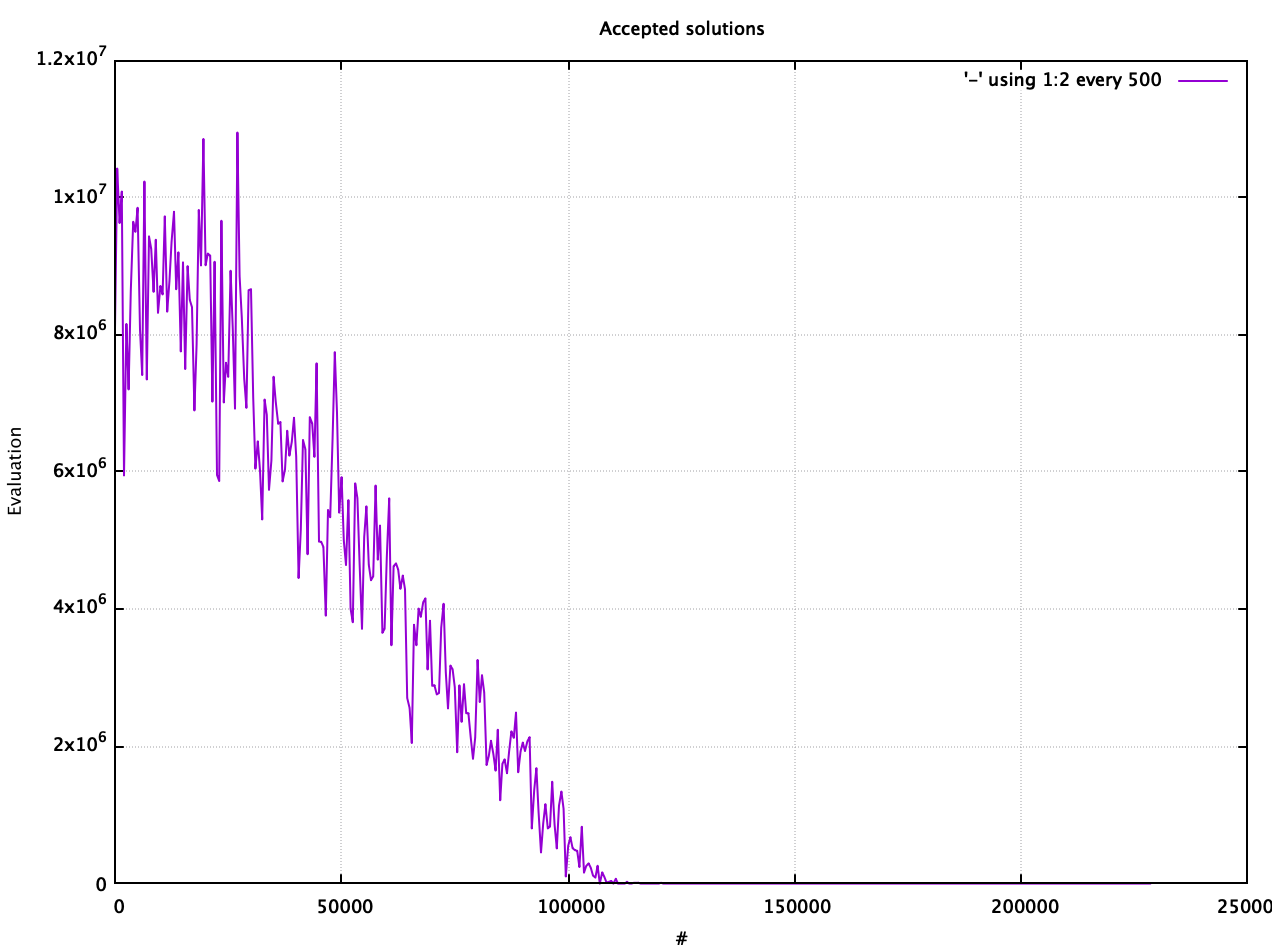
\includegraphics[width=\linewidth]{1.png}
    \label{fig:1}
\end{figure}

La gráfica muestra cómo la evaluación de las soluciones descienden conforme el algoritmo progresa y cómo permite que la evaluación aumente, pasando a una solución peor.
\par
El sistema sólo acepta soluciones peores mientras la temperatura lo permita; en la gráfica se puede apreciar que la diferencia de las evaluaciones es cada vez menor, hasta llegar a un punto donde es casi nula.
\par
\bigskip
Aumentar el tamaño de los lotes provoca una mejor exploración del espacion de búsqueda, aumentando la probabilidad de obtener una buena solución, sin embargo, el tiempo de ejecución del algoritmo también aumenta en relación al tamaño de lote, ya que se intenta mejorar la solución actual L veces, hasta un máximo de M sin mejora.
\par
La siguiente figura pertenece a una instancia de TSP con 40 ciudades, $L = 6000, M = L\times3, \varepsilon = 0.01, \varphi = 0.95$.

\begin{figure}[H]
    \centering
    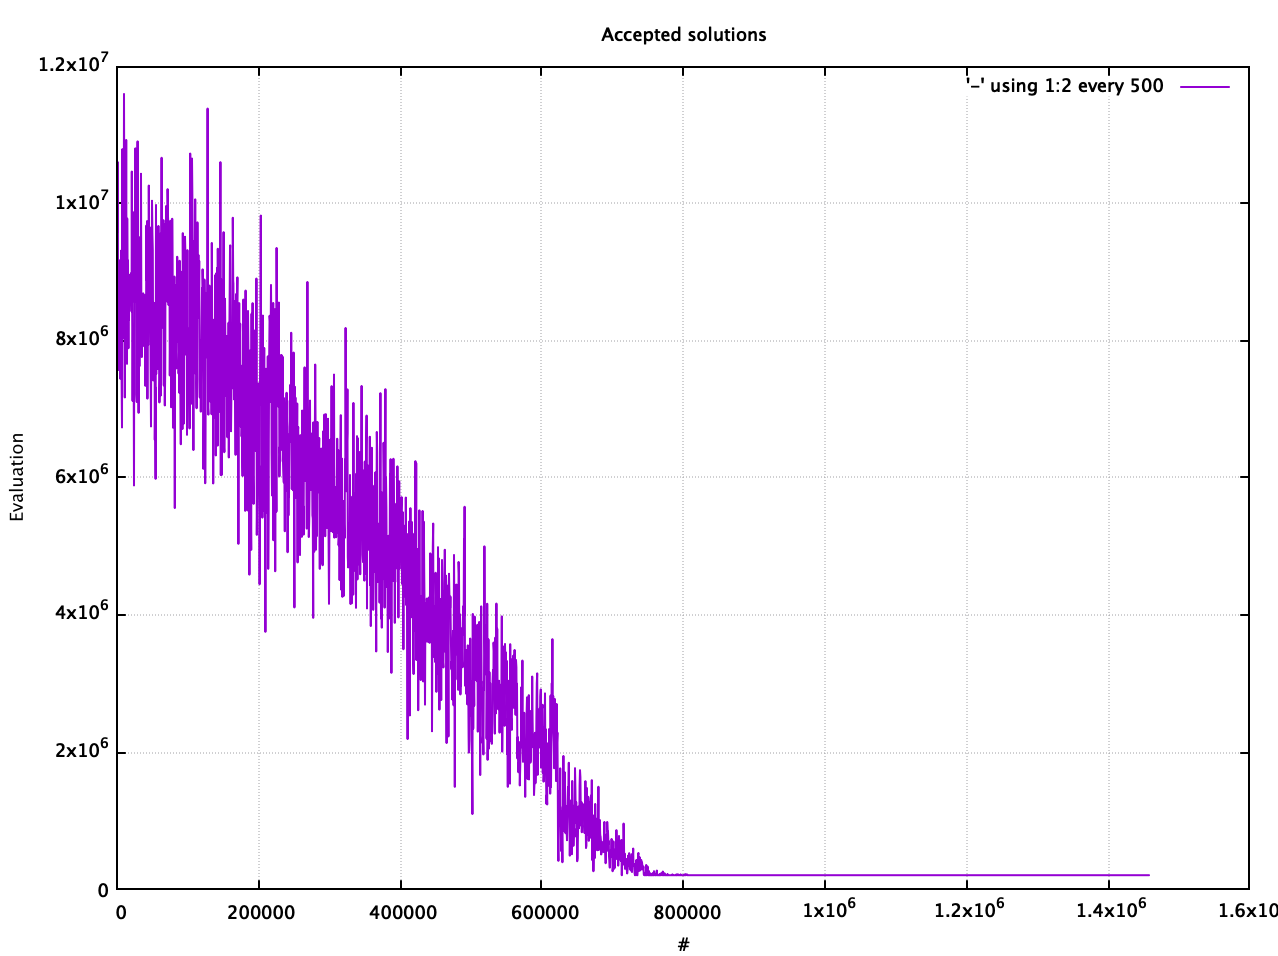
\includegraphics[width=\linewidth]{2.png}
    \label{fig:2}
\end{figure}

El factor de enfriamiento también altera de forma directa el tiempo de ejecución del algoritmo, ya que miengras más cercana sea a 1, se realizan muchas más iteraciones antes de cumplir la condición de terminación.
\par
La siguiente figura pertenece a una instancia de TSP con 40 ciudades, $L = 6000, M = L\times3, \varepsilon = 0.01, \varphi = 0.99$.

\begin{figure}[H]
    \centering
    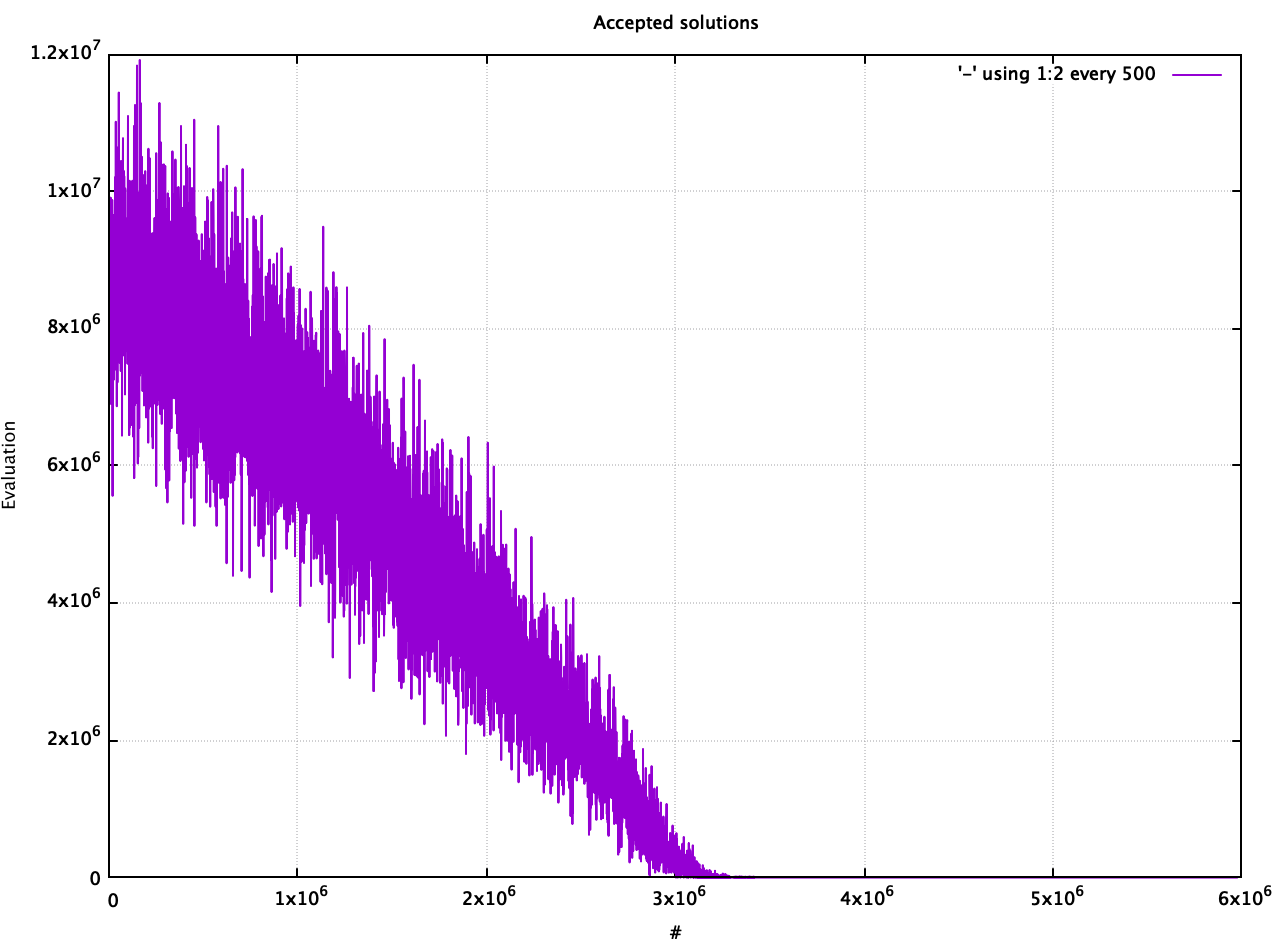
\includegraphics[width=\linewidth]{3.png}
    \label{fig:3}
\end{figure}

En los 3 casos, al probar con diferentes semillas, la mejor solución encontrada, resultó ser la misma permutación de ciudades, lo que sugiere que el ajuste de parámetros no afecta en gran medida para instancias pequeñas del problema.
\par
Sin embargo en instancias más grandes, como 150 ciudades, es escencial la experimentación en el ajuste de parámetros para conseguir mejores soluciones.

\begin{thebibliography}{2}
\bibitem{1} 
Kirkpatrick, S.; Gelatt Jr, C. D.; Vecchi, M. P. (1983). \textit{Optimization by Simulated Annealing}
\bibitem{2} 
Applegate, D. L.; Bixby, R. M.; Chvátal, V.; Cook, W. J. (2006), \textit{The Traveling Salesman Problem}
\end{thebibliography}
\end{document}
